\documentclass[11pt, notitlepage,  letterpaper]{article}


%% Horizontal Lengths - Max 6.5
\setlength{\footskip}{0.5in}
\setlength{\hoffset}{0in}
\setlength{\oddsidemargin}{-.2in}
\setlength{\evensidemargin}{-.2in}
%\setlength{\textwidth}{6.9in}
\setlength{\textwidth}{6.6in}

%% Vertical Lengths - Max 9.0
\setlength{\headheight}{0in} \setlength{\topskip}{0in}
\setlength{\voffset}{0in} \setlength{\topmargin}{0.5in}
\setlength{\textheight}{8.4in}

%\usepackage{fancyheadings}

\usepackage{url}
\usepackage[]{epsfig,amsmath}[]


%\pagestyle{headings}
%\pagestyle{fancy}
\pagenumbering{arabic}


%%%%%%%%%%%%%%%%%%%%%%%%%%%%%%%%%%%%%%%%%%%%%%%%%%%%%%%%%%%%%%%%%%%%%%
% New definitions and commands
\newtheorem{define}{Definition}[section]
\newtheorem{theorem}[define]{Theorem}
\newtheorem{question}[define]{Question}
\newtheorem{problem}[define]{Problem}


%**************************************


\begin{document}
\title{
{Solving Two-dimensional Forward Problems on an Annulus}\\{Using
Spectral Fourier Methods}}

\vfill
\author{S.\ Choe \\ skchoe@cs.utah.edu \and R.\ M.\ Kirby \\ kirby@cs.utah.edu}

\renewcommand{\today}{Jan 30th, 2004}

\maketitle

\begin{abstract}
In this report, we present a spectral Fourier method for solving a
Poisson equation with Dirichlet and Neumann boundary conditions
respectively on an annulus domain. By using the tensor product
between spectral and Fourier bases, we could apply the high-order
method on the annulus domain. The fast Fourier transform allowed
the rapid convergence on the radius to be maintained to all
angular direction on the annulus.
\end{abstract}

%\noinden {\bf Keywords: Spectral Element Methods, Poisson Equation}

\tableofcontents

%-------------------------------------------------------------------------------
\clearpage

\section{Introduction}

%\{ {\it  sp1d\_ch1.tex} \}

Spectral method is a numerical scheme to approximate and simulate
the solution of partial differential equations. It has developed
rapidly in the past three decades and been applied to many field
in numerical simulation.

One of main reasons that it has gained broad and fast acceptance
is that it can take various system of infinitely differentiable
basis functions as trial functions, for instance, we can use the
representation of a function $u$ throughtout the domain via a
truncated serier exansion as follows:
\begin{equation}
\label{solapprx}
u \approx u_N = \sum_{n=0}^{N} \hat u_n \phi_n,
\end{equation}
where $\phi_n$ are the basis functions. In general this basis
functions may be the Chebyshev polynomials $T_n$ or the Legendre
polynomials $L_n$ or another member of the class of Jacobi
polynomials $P_n^{\alpha, \beta}$. By choosing an appropriate
orthogonal system based on its domain of orthogonality, we can
apply the method to problems such as periodic/non-periodic
problems and problems defined on compact domain, half/all
intervals.


Spectral methods can be classified into 2 parts in its
characteristics. We call them to be nodal and modal method,
respectively.
\begin{itemize}
\item The nodal method is usually called as pseudo-spectral or
collocation methods. The coefficients $\hat u_n$ of
(\ref{solapprx}) are obtained by requiring  the residual function
to be zero exactly at grid that is a set of nodes.

\item The modal method is associated with the method of weighted
residuals where the residual function is weighted with a set of
test functions and after integration is set to zero. In our
formulation we bring in the Galerkin method which has test
functions same as the basis functions.
\end{itemize}

In the collocation approach the coefficients represent the nodal
value of the physical variable unlike the Galerkin method.

The other thing which is so fascinating is its high accuracy and
convergence. In particular, the spectral polynomial method
facilitates the control of the resolution of element size and the
order of approximation. This enables the method to converge in
exponential speed which shows a noticeable difference from
classical finite difference and other purely element methods.
Unlike finite elements and finite difference, the order of
convergence is not fixed and it is related to the maximum
regularity of the solution.

In this report, I investigate the spectral polynomial method and
Fourier method for solving a partial differential equation
specific to the forward Poisson problem with Dirichlet and Neumann
boundary condition on inner and outer boundary circles
respectively. Throughout the report, I will  formulate our
approach that utilizes spectral polynomial element and Fourier
method in tensor product form. As an conclusion we present the
result of numerical solution and its convergence by h/p adaptive
control.


\section{The Numerical Solution of Poisson Equation on a 2-dimensional Annulus}
%\{ {\it  sp1d\_ch2.tex} \}

\subsubsection{Poisson Equation in Polar Coordinates and Basis Functions}

We formulate the Generalized Poisson problem on an annulus $[a, b]\times[0, 2\pi]$, $a > 0$ under the periodic solution $u$ as follows:
\begin{eqnarray}\label{genpois}
-\left[\frac{\partial}{\partial r} (\sigma(r,\theta) \frac{\partial}{\partial r}) + \frac{1}{r} (\sigma(r,\theta) \frac{\partial}{\partial r}) + \frac{1}{r^2}\frac{\partial}{\partial \theta} (\sigma(r,\theta)  \frac{\partial}{\partial \theta})\right] u(r, \theta) = f(r, \theta),\\
\mbox{with periodicity of }u, \;\;\; u(r,0) = u(r,2\pi),
\end{eqnarray}
where $r \in [a, b]$ and $\theta \in [0, 2 \pi]$.

The boundary conditions for this domain is given by:
\begin{equation}
u(a,\theta) = {\mathcal G}_D(\theta), \hspace{1in} \frac{\partial}{\partial r} u(b,\theta) = {\mathcal G}_N(\theta),
\end{equation}
where $\theta \in [0,2\pi]$.

\vspace{0.1in}
The representation of approximation of $u$ is guaranteed by Weierstrass theorem:
\begin{equation}\label{truncapp}
u(r,\theta) = \sum_{j=0}^{N_r} \sum_{k=-N_\theta/2+1}^{N_\theta/2} \hat{u}_{jk} \phi_j(r) e^{ik\theta},
\end{equation}
where $r \in [a, b]$ and $\theta \in [0, 2 \pi]$ for the global degree of freedom $N_r$ and $N_{\theta}$ on $\hat{u}_{jk}$'s.

\vspace{0.1in}

The basis functions $\{\phi_j\}_{j=0}^{N_r}$ shown at linear span
(\ref{truncapp}) are defined as modified Jacobi polynomials
defined in \cite{Karniadarkis}.

\vspace{0.1in}
As a review of discrete Fourier transform in $N$-point grid described in \cite{Trefethen}, the formula for the discrete Fourier transform for $\{v_j\}$ is
\begin{equation}
\hat{v}_k = h \sum_{j=1}^{N} e^{-ikx_j}v_j, \;\; k = -\frac{N}{2}+1, \ldots , \frac{N}{2},
\end{equation}
where $x_j = j\frac{2\pi}{N}$ and the inverse discrete Fourier transform for $\{\hat{v}_k\}$ is given by
\begin{equation}
v_j = \frac{1}{2\pi}\sum_{k = -N/2+1}^{Nr/2}e^{ikx_j}\hat{v}_k,\;\; j = 1, \ldots, N.
\end{equation}


\subsubsection{Formulation of Spectral Polynomial and Fourier Methods}

In this project, we assume the conductivity term $\sigma$ in
equation (\ref{genpois}) to be only dependent on variables showing
the radius domain as we multiply $r^2$ in each side of equation
(\ref{genpois}). Then the Poisson equation in polar coordinate is
as follows:
\begin{eqnarray}
-\left[r^2 \frac{\partial}{\partial r} (\sigma(r) \frac{\partial}{\partial r}) + r \sigma(r) \frac{\partial}{\partial r} + \sigma(r) \frac{\partial^2}{\partial \theta^2}\right] u(r, \theta) = r^2 f(r, \theta).
\end{eqnarray}

\vspace{0.1in}

We utilize the Galerkin method, with test functions of the form:
\begin{equation}
\phi_p(r) e^{iq\theta}, \hspace{.5in} p=0,\ldots,N_r, \;\; q = -\frac{N_\theta}{2}+1,\ldots,\frac{N_\theta}{2}.
\end{equation}

\vspace{0.1in}

The weak form of the equation is as follows:
\begin{equation}\label{galeqn}
-\langle  r^2 \frac{\partial}{\partial r} (\sigma \frac{\partial}{\partial r}u) + r \sigma \frac{\partial}{\partial r}u + \sigma \frac{\partial^2}{\partial \theta^2}u, \phi_p e^{iq\theta} \rangle = \langle r^2 f, \phi_p e^{iq\theta} \rangle.
\end{equation}

\vspace{0.1in} Define $T_i, i = 1,\ldots,4$ as follows
\begin{eqnarray}
T_1 &=& \int_{0}^{2\pi} \int_{a}^{b} \phi_p e^{iq\theta} r^2 \frac{\partial}{\partial r}\left[\sigma(r) \frac{\partial}{\partial r}u(r, \theta)\right] dr d\theta,\\
T_2 &=& \int_{0}^{2\pi} \int_{a}^{b} \phi_p e^{iq\theta} r \sigma(r) \frac{\partial}{\partial r}u(r, \theta) dr d\theta,\\
T_3 &=& \int_{0}^{2\pi} \int_{a}^{b} \phi_p e^{iq\theta} \sigma(r) \frac{\partial^2}{\partial \theta^2}u(r, \theta) dr d\theta,\\
\mbox{and} \hspace{.5in}T_4 &=& \int_{0}^{2\pi} \int_{a}^{b} \phi_p e^{iq\theta} r^2 f(r, \theta) dr d\theta
\end{eqnarray}

Then equation (\ref{galeqn}) becomes:
\begin{equation}\label{smpeqn}
- T_1 - T_2 - T_3 = T_4.
\end{equation}

We obtain boundary terms by integrating by parts on $T_1$ as
follows:
\begin{eqnarray}
T_1 &=& \int_0^{2\pi}e^{iq\theta} \left[ r^2\sigma(r)\frac{\partial}{\partial r}u(r,\theta)\phi_p(r)\right]_a^b d\theta \\
&-&2 \int_0^{2\pi}\int_a^b e^{iq\theta} r \sigma(r)\frac{\partial}{\partial r}u(r,\theta)\phi_p(r)drd\theta \\
&-& \int_0^{2\pi}\int_a^b e^{iq\theta} r^2\sigma(r)\frac{\partial}{\partial r}u(r,\theta) \frac{d}{dr}\phi_p(r)drd\theta.
\end{eqnarray}

Then the right hand side of (\ref{smpeqn}) becomes
\begin{eqnarray}\label{rhseqn1}
- T_1 - T_2 - T_3 &=& - \int_0^{2\pi}e^{iq\theta} \left[ r^2\sigma(r)\frac{\partial}{\partial r}u(r,\theta)\phi_p(r)\right]_a^b d\theta \\
&+& \int_0^{2\pi}\int_a^b e^{iq\theta} r \sigma(r) \frac{\partial}{\partial r}u(r,\theta)\phi_p(r)drd\theta \\
&+& \int_0^{2\pi}\int_a^b e^{iq\theta} r^2 \sigma(r) \frac{\partial}{\partial r}u(r,\theta) \frac{d}{dr}\phi_p(r)drd\theta \\
&-& \int_0^{2\pi}\int_a^b e^{iq\theta} \sigma(r) \frac{\partial^2}{\partial \theta^2}u(r, \theta) \phi_p(r) dr d\theta
\end{eqnarray}

Using (\ref{truncapp}) and the orthogonal properties of
$\{e^{ik\theta}\}$, $k =
-\frac{N_\theta}{2}+1,\ldots,\frac{N_\theta}{2}$, we can simplify
(\ref{rhseqn1}) to obtain:

\begin{eqnarray}\label{rhseqn2}
- T_1 - T_2 - T_3 &=& - \int_0^{2\pi}e^{iq\theta} \left[ r^2\sigma(r)\frac{\partial}{\partial r}u(r,\theta)\phi_p(r)\right]_a^b d\theta \\
&+& 2\pi \sum_{j=0}^{N_\theta} \hat{u}_{jq} \int_a^b r \sigma(r) \frac{d}{dr} \phi_j(r) \phi_p(r) dr \\
&+& 2\pi \sum_{j=0}^{N_\theta} \hat{u}_{jq} \int_a^b r^2 \sigma(r) \frac{d}{dr} \phi_j(r) \frac{d}{dr}\phi_p(r) dr \\
&+& 2\pi \sum_{j=0}^{N_\theta} \hat{u}_{jq} q^2 \int_a^b \sigma(r) \phi_j(r) \phi_p(r) dr.
\end{eqnarray}


Let us define the following matrices:
\begin{eqnarray}
({\bf M}_1)_{jp} & = & \int_a^b r \sigma(r) \frac{d}{dr} \phi_j(r) \phi_p(r) \;dr  \\
({\bf M}_2)_{jp} & = & \int_a^b r^2 \sigma(r) \frac{d}{dr} \phi_j(r) \frac{d}{dr} \phi_p(r) \;dr  \\
({\bf M}_3)_{jp} & = & \int_a^b \sigma(r) \phi_j(r) \phi_p(r) \; dr,
\end{eqnarray}
where $j, p = 0, \ldots, N_\theta$.

$T_4$ becomes:

\begin{eqnarray}
T_4 &=& \int_a^b \int_0^{2\pi} \phi_p(r) e^{iq\theta} r^2 f(r,\theta) d\theta dr \\
    &=& \int_a^b r^2\phi_p(r) \int_0^{2\pi} f(r,\theta) e^{iq\theta} d\theta dr \\
\end{eqnarray}

For given $r$, the Discrete Fourier Transform for $f(r, \theta)$ is defined by
\begin{equation}
f(r, \theta_\tau) = \frac{1}{2\pi} \sum_{k=-N_\theta/2+1}^{N_\theta/2} e^{ik\theta_\tau} \widehat{f(r)}_k
\end{equation}

where
\begin{equation}
\widehat{f(r)}_k = \frac{2\pi}{N_\theta} \sum_{j=1}^{N_\theta} e^{-ik\theta_j} f(r, \theta_j)
\end{equation}
with $ k \in \{-\frac{N_\theta}{2}+1, \cdots, \frac{N_\theta}{2}\}$ and $\theta_j \in \{ \frac{2\pi}{N_\theta}, \cdots, 2\pi  \}$.

Then:
\begin{center}
\begin{eqnarray}
T_4&=& \int_a^b r^2\phi_p(r) \int_0^{2\pi} \frac{1}{2\pi} \sum_{k=-N_\theta/2+1}^{N_\theta/2} e^{ik\theta} \widehat{f(r)}_k e^{iq\theta} d\theta dr \\
%&=& \int_a^b r^2\phi_p(r) \sum_{k=-N_\theta/2+1}^{N_\theta/2} \widehat{f(r)}_k \frac{1}{2\pi} \int_0^{2\pi}  e^{ik\theta} e^{iq\theta} d\theta dr \\
%&=& \int_a^b r^2\phi_p(r) \sum_{k=-N_\theta/2+1}^{N_\theta/2} \widehat{f(r)}_k \delta_{k,q} dr\\
&=& \int_a^b r^2\phi_p(r) \widehat{f(r)}_q dr.
%&=& \sum_\sigma w_\sigma r_\sigma^2\phi_p(r_\sigma) \widehat{f(r_\sigma)}_q.
\end{eqnarray}
\end{center}


\begin{eqnarray}
 2\pi \sum_{j=0}^{N_\theta} \hat{u}_{jq} {M_1}_{jp}
+ 2\pi \sum_{j=0}^{N_\theta} \hat{u}_{jq} {M_2}_{jp} + 2\pi
\sum_{j=0}^{N_\theta} \hat{u}_{jq} q^2 {M_3}_{jp} = \int_a^b
r^2\phi_p(r) \widehat{f(r)}_q dr \\
+ b^2\sigma(b) \phi_p(b) \int_0^{2\pi}e^{iq\theta} {\mathcal
G}_N(\theta) d\theta - a^2\sigma(a) \phi_p(a)
\int_0^{2\pi}e^{iq\theta} \frac{\partial}{\partial r}u(a,\theta)
d\theta
\end{eqnarray}
where $j, p = 0, \ldots, N_r$.

We apply the Fourier transform to the integral term with
${\mathcal G}_N$ and the same idea as one-dimensional case to each
term about boundary conditions.


\section{Experiment Results}
%\{ {\it  sp1d\_ch3\_1.tex} \}

\subsection {H/P Convergence Test for Two-dimensional Solution}

In this section we present the result of convergence in both $h$ refinement and $p$ refinement with the following steady-state Poisson differential equation:
\begin{equation}
\label{pois_sin}
-r^2 \frac{\partial}{\partial r} (\sigma \frac{\partial}{\partial r}u) - r \sigma \frac{\partial}{\partial r}u - \sigma \frac{\partial^2}{\partial \theta^2}u = r \cos \theta \left[ -4 r \pi \cos S_r + \{4\pi^2 + 1\} \sin S_r \right],
\end{equation}
for all $r \in [1, 2], \theta \in [0, 2\pi]$ with $\sigma(r) = r$. The analytic solution is known as 
\begin{equation}
u(r, \theta) = \sin S_r \cos \theta,
\end{equation}
where $S_r = 2\pi (r-1) - \pi$.

The numerical and exact solutions by the solver we developed is shown in figure (\ref{sinsol}).

\begin{figure}[h]
    \begin{center}
    \epsfig{file = figs_dn/sinDN_e10_t8.eps, width = 5cm} %Error: 4.7740e-15
    \epsfig{file = figs_dn/sinDN_e10_t8_1.eps, width = 5cm}
    \caption{\label{sinsol}Numerical and exact solution of equation (\ref{pois_sin}) with polynomial order $P=10$, $10$ equidistance elements. This gives the error 4.7740e-15 to the exact solution}
    \end{center}
\end{figure}

\begin{figure}[h]
    \begin{center}
    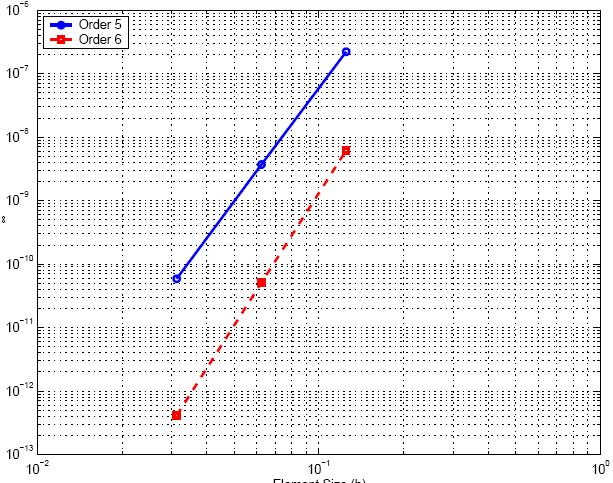
\epsfig{file = figs_dn/sinDNhconv.eps, width = 8.3cm}
    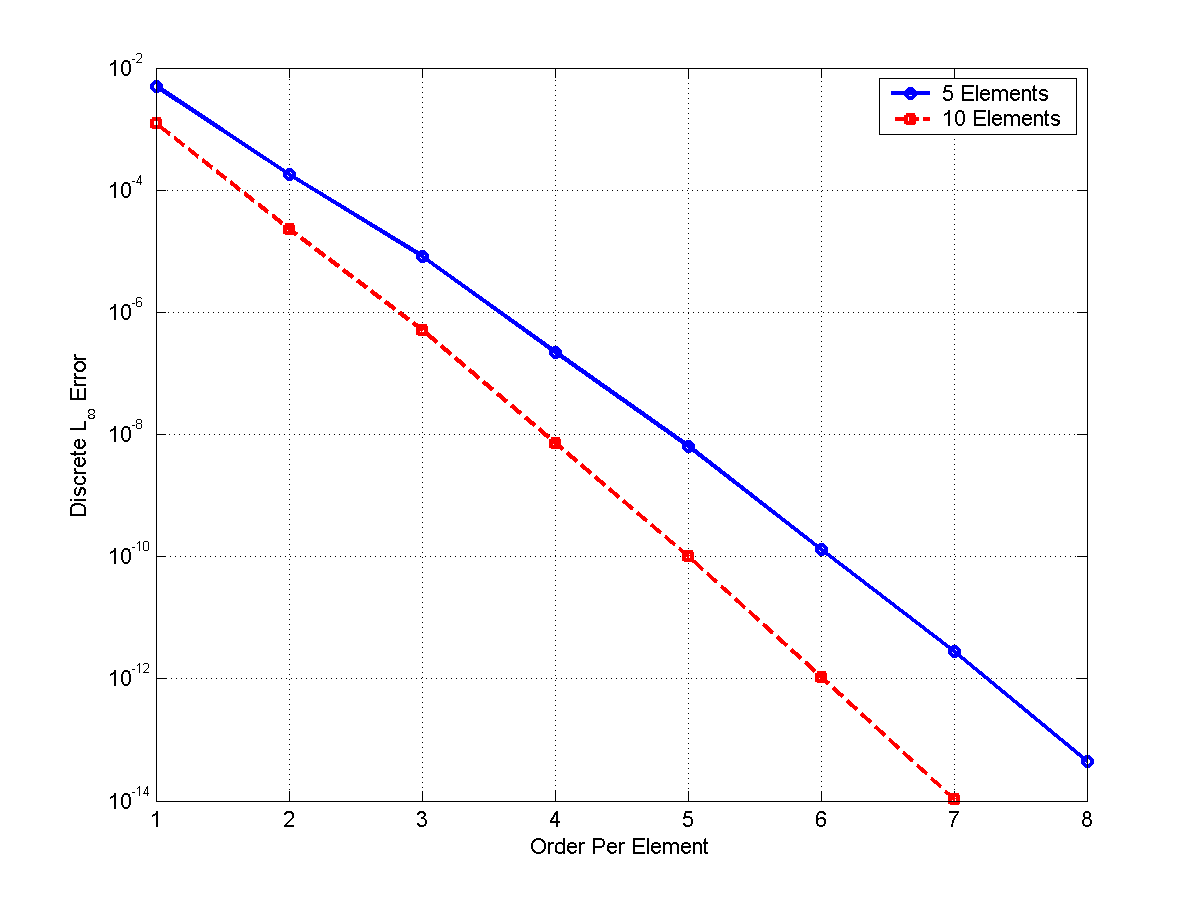
\epsfig{file = figs_dn/sinDNpconv.eps, width = 8.3cm}
    \caption{\label{sinDNconv}
(Left)Convergence with respect to discrete $L^{\infty}$ norm as a function of size of elements. This test is performed using the h-type extension with fixed polynomial order 5 and 6 respectively. Error on the Log-Log axis is demonstrating the algebraic convergence of the h-type extension.
(Right)Convergence w.r.t. $L^{\infty}$ norm as a function of size of polynomial order in semi-Log plot. It shows the exponential convergence of p-type extension for smooth solution. Two tests are performed for p-type extension with element length $0.2$ and $0.1$.
}
\end{center}
\end{figure}


\begin{table}[h]
\centering \caption{\label{hconv2t} This table shows the convergence of h-type (left) and p-type (right) resolution control done above Figure (\ref{sinDNconv}). We can see the slopes of each order $P$ is $P+1$ }
\begin{tabular}{|c|c|c|} \hline
    Polynomial order&Error($L^{\infty}$)&Slope   \\ \hline \hline
    5&$9.3603e-013$ &$5.9406$ \\ \hline
    6&$8.6542e-014$ &$6.9402$ \\ \hline
\end{tabular}
\hspace{.5in}
\begin{tabular}{|c|c|} \hline
    Element Size&Error($L^{\infty}$)\\ \hline
    0.2&$1.9385e-012$  \\ \hline
    0.1&$3.4611e-013$  \\ \hline
\end{tabular}

\end{table}

%\{ {\it  sp1d\_ch3\_2.tex} \}

\subsubsection {High order Polynomial Solution and Its Convergence}

In this section we construct a polynomial $P_n$ of order $n$ defined on $[0,1]$, which satisfies the following.
\begin{eqnarray}
\label{pois_scrv}
    P_n(0) = 0, &P_n(1) = 1 \\
    \frac{d^k}{dx^k}P_n(0) = 0, &\frac{d^k}{dx^k}P_n(1) = 0
\end{eqnarray}
for all $k = 1, \cdots, n-2$. \\
For each $n$, we obtain polynomial $P_n$ by solving a system of
linear equations that determines the set of coefficients of $P_n$.
We use the spectral polynomial solver to approximate the second
derivative $Q_{n-2}$ of $P_n$.

\begin{figure}[h]
    \begin{center}
    \epsfig{file = Doc-Report_Fwd2D/figs_dn/ScrvH5_A.eps, width = 5cm}
    \epsfig{file = Doc-Report_Fwd2D/figs_dn/ScrvH5_N.eps, width = 5cm}
    \caption{\label{scrvsol}Example of curve that satisfies conditions (\ref{pois_scrv}) with polynomial order $n=7, 9, 12, 14, 15$. The error is $2.9239e-8$}
    \end{center}
\end{figure}

We investigate the convergences by the h-type, p-type extension of
trial functions below.

\begin{problem}
Consider the following differential equation for $u(x)$ such that
\begin{equation}
\label{poi_poly}
-r^2 \frac{\partial}{\partial r} (\sigma \frac{\partial}{\partial r}u) - r \sigma \frac{\partial}{\partial r}u - \sigma \frac{\partial^2}{\partial \theta^2}u = e^{-(r-1)^2}\{P_n(r) + (2r^2(r-1)-r)P_n'(r) - r^2 P_n''(r)\} \cos \theta,
\end{equation}
for all $r$ in $[0.1, 1.1]$ with $\sigma(r) = e^{-(r-1)^2}$.

The exact solution is known to be:
\begin{equation}
u(r, \theta) = P_n(r) \cos \theta
\end{equation}
where $r$ in $[0.1, 1.1]$ and $\theta$ in $[0, 2\pi]$.
\end{problem}

\begin{figure}[h]
\begin{center}
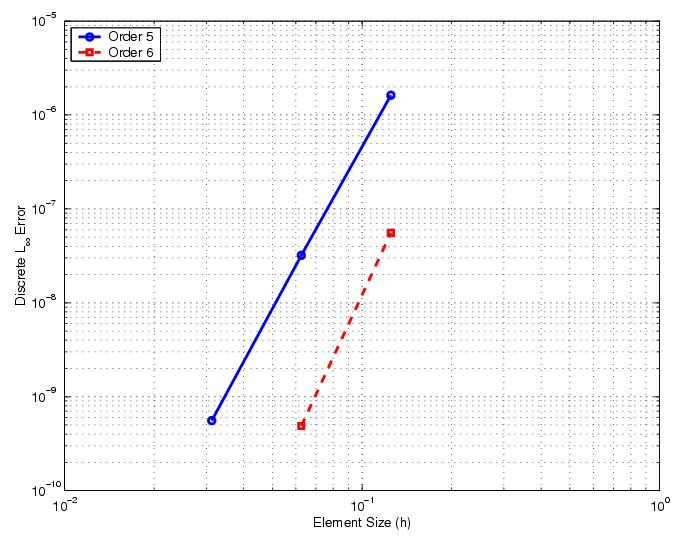
\epsfig{file = Doc-Report_Fwd2D/figs_dn/ScrvHconv.eps, width =
8.3cm} 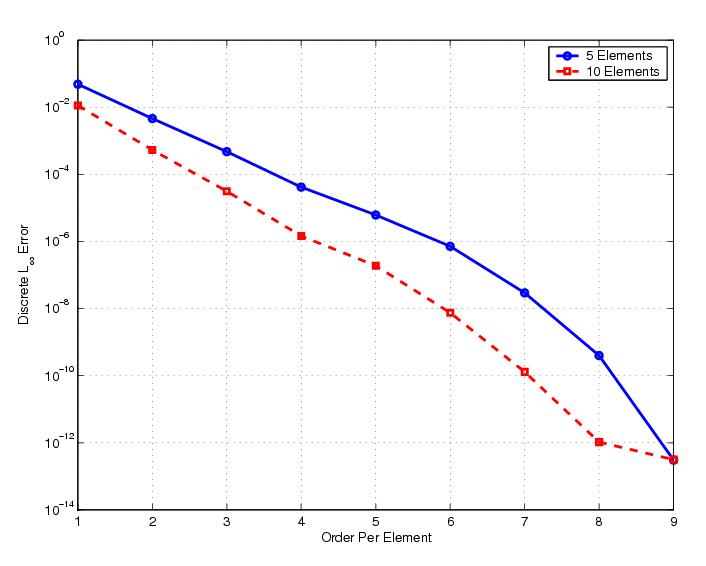
\epsfig{file = Doc-Report_Fwd2D/figs_dn/ScrvPconv.eps,
width = 8.3cm} \caption{\label{ScrvconvDN} (Left) Convergence with
respect to discrete $L^{\infty}$ norm as a function of size of
elements. This test is performed using the h-type extension with
fixed polynomials of order 3, 4, and 5 respectively. Error on the
Log-Log axis demonstrates the algebraic convergence of the h-type
extension. (Right) Convergence w.r.t. $L^{\infty}$ norm as a
function of size of polynomial order in semi-Log plot. It shows
the exponential convergence of p-type extension for smooth
solutions. The two tests are performed for p-type extension with
element lengths of $0.2$ and $0.1$. }
\end{center}
\end{figure}

\begin{table}[h]
\centering \caption{\label{hconv2t} This table shows the
convergence of h-type resolution control done above Figure
(\ref{ScrvconvDN}). We can see the slopes of each order $P$ is
$P+1$ }
\begin{tabular}{|c|c|c|} \hline
    Polynomial order&Error($L^{\infty}$)&Slope   \\ \hline \hline
    5&$8.5305e-012$ &$5.7556$ \\ \hline
    6&$4.7180e-012$ &$6.8332$ \\ \hline
\end{tabular}
\hspace{.5in}
\begin{tabular}{|c|c|} \hline
    {Element Size}&Error($L^{\infty}$) \\ \hline \hline
    0.2&$9.0616e-13$  \\ \hline
    0.1&$9.4747e-13$ \\ \hline
\end{tabular}
\end{table}


\section{Conclusion}
%\clearpage
%\{ {\it  sp1d\_ch4\_1.tex} \}

In 2-dimensional case, we looked into the theory of Spectral
Polynomial and Fourier Method and its solvability. We also
investigated the feature of convergence in the viewpoint of h/p
convergence property in comparison to classical finite element
method. By using Galerkin method, we could incorporate the weak
solution and get the problem to be changed to system of linear
equations which we can solve it by computer.

By implementing the Spectral element solver for one dimensional Poisson equation having Dirichlet and Neumann boundary conditions, we could experiment all the theory with various specific cases of high-order solutions which were hard to get acceptable convergence in a given time and resolution of domain.


%------------------------------------------------------------------------------
%   BIBLIOGRAPHY
%\clearpage

%\{ {\it  sp1d\_chbib.tex} \}

\begin{thebibliography}{9}

\bibitem{Karniadarkis}{\bf Spectral/Hp Element Methods for Cfd},
        George Em Karniadakis, Spencer J. Sherwin, \/
        Oxford Univ Press, 1999.

\bibitem{Trefethen}{\bf Spectral Methods in MATLAB},
        Lloyd N. Trefethen, \/
        Society for Industrial and Applied Mathematics, 2001.

\bibitem{Johnson}{\bf Lecture note of Advanced Methods in Scientific
Computing},
        Christopher R. Johnson, \/
        School of Computing, University of Utah, 2002.

\bibitem{Chen}{\bf A direct spectral collocation Poisson solver in polar and cylindrical
coordinates},
        Chen HL. Su YH. and Shizgal BD., \/
        Journal of Computational Physics. 160(2), 453-469 (2000).

\bibitem{Choe}{\bf Solving One-dimensional Forward Problems using Spectral Element
Method},
        S. Choe, \/
        Project report in Computational Engineering and Science Program, University of Utah, 2004.


\end{thebibliography}



%-------------------------------------------------------------------------------
%   APPENDIX
%
%

\{ {\it  sp1d\_chapdx.tex} \}

%\clearpage
\appendix
\section {Gaussian Quadrature Formula}



\end{document}
